\chapter{C言語入門}

\noindent
プログラミング言語とは、コンピューターに仕事をさせるために、その作業内容を指示するための特別な言語である。この言語で書かれた作業の手順書を「プログラム」とよび、プログラムを作成することを「プログラミング」という。
プログラミング言語には、さまざまな種類がある。C言語はもともと、UNIX (マルチユーザ、マルチタスクのオペレーティングシステム)を記述するためのシステム言語として開発された。現在は、システムソフトウエアの作成だけでなく、事務処理や科学技術計算、アプリケーションソフトウエア(表計算やワープロなど)の開発など、広く汎用プログラミング言語として使用されている。

\section{C言語の基礎知識}
\label{sec:C:basic}
\subsection{まずはコンパイル}

ここでは、最も短い``コンパイル可能なCのプログラム''を作成し、それをコンパイルしてみよう。

\clangpara{プログラムの構成}
Cのプログラムの最小単位は関数である。``Cのプログラムは関数を並べたものである''ということもできる。
関数を定義するときは以下のように書く。
\begin{quote}
  \begin{verbatim}
  型 関数名(引数) { 処理 }
  \end{verbatim}
\end{quote}
\begin{description}
\item[関数名] 関数の名前は自由につけられる。ここで、Cでプログラム中に使う名前(関数以外でも)は
  \begin{itemize}
  \item 先頭は英字または \verb+_+ (下線)
  \item 2文字以降は英数字または \verb+_+ (下線)
  \item 大文字/小文字は区別される
  \end{itemize}
\item[引数] 関数には引数(パラメタ)を渡すことができる。(具体的な例については\ref{sec:C:function}節参照)
\item[型] 関数は何かを処理して最後に値を返す(関数値)。この関数値の種類を示す。
\item[処理] この中で、1) 関数が行う処理内容を書き、2) 最後に関数値を返す。
  関数値を返すには
  \begin{quote}
\begin{verbatim}return 関数値;
\end{verbatim}
  \end{quote}
  と書く。
\end{description}
プログラム中に関数は複数作ることができるが、必ず\verb+main+という関数が必要である。(すべての処理は \verb+main+ から始まる。) 以上をふまえて、Cの関数の例を示す。
\begin{reidai}\label{ex:hinagata1}
\begin{verbatim}
int main() { return 0; }
\end{verbatim}
\end{reidai}

\clangpara{コンパイル}
Emacsなどのテキストエディタを使って例\ref{ex:hinagata1}の1行を入力したテキストファイルを作成し、\ref{ex:hinagata1}cという名前で保存する。このプログラムをコンパイルするには \verb+gcc+ を用いる。
\begin{commandline2}
\prompt \underline{gcc \ref{ex:hinagata1}c}
\end{commandline2} \noindent
同一ディレクトリに{\tt a.out}というファイルができているので、以下のように実行する。
\begin{commandline2}
\prompt \underline{./a.out}
\end{commandline2} \noindent
(ただし、現段階のプログラムでは、実行してももちろん何も起こらない。)

\subsection{書式の慣例}

先に進む前に、Cのプログラムの書式の慣例について、いくつか説明する。

\clangpara{自由書式 (free format)}
C言語では、1つの行に複数の文を書いたり、または1つの文を複数の行に書くことができる(自由書式)。
文の終わりは、記号 \verb+;+ で判別する。
\begin{quote}
  1つの行に2つの文を書く
\begin{verbatim}
aaaaa; bbbbbbb;
\end{verbatim}
  1つの文を2つの行にわけて書く
\begin{verbatim}
aaaaaaaa
aaaaaaa;
\end{verbatim}
\end{quote}
例えば、例\ref{ex:hinagata1}は、以下のようにも書くことができる。
\begin{reidai}\label{ex:hinagata2}
\begin{verbatim}
int main() {
  return 0;
}
\end{verbatim}
\end{reidai} \noindent
本書では、例\ref{ex:hinagata2}のような書式を用いることにする。スペース節約のため空行は入れないが、実際のコードでは適宜空行を挟むことでプログラムの可読性が向上する。

\clangpara{インデントの慣例}
Cの文は、意味上のレベル(入れ子構造の階層)を持つ。意味上の各レベルをわかりやすくするため、より深いレベルを右側に段付けして書くのがよい(インデント)。
\begin{quote}
\begin{verbatim}
  aaaaa          /* ← 最上位のレベルの文 */
  aaaaa
    bbbbb        /* ← 1つ深いレベルの文 */
    bbbbb
      ccccc      /* ← もう1つ深いレベルの文 */
      ccccc
    bbbbb
  aaaaa
\end{verbatim}
\end{quote}
例\ref{ex:hinagata2}の関数は、すでにインデントして書かれている。
インデントは上の行から行毎に順にキーボード上の \tabkey を押せばできる。
だたし、Emacs の場合は \verb+c-mode+ になっている必要がある。
\verb+c-mode+ になっている場合は、Emacs の下の部分に \verb+(C)+ と表示されている。
\verb+c-mode+ にするには、\esckey を押して(離し)、
\verb+x+ を押して(離し)、\verb+c-mode+ と入力して \ret を押せばよい。
\clangpara{コメント}
\verb+/*+ と \verb+*/+ で囲った部分はコメントとみなされる(複数行も可)。
例えば、例\ref{ex:hinagata2}にコメントを挿入してみると、
\begin{reidai}
\begin{verbatim}
int main() {
  /* これもコメント。
     複数行にわたっても OK。 */
  return 0;
}
\end{verbatim}
\end{reidai} \noindent
\verb+/*+ と \verb+*/+ の間にある部分はコンパイルするときは無視される。

\subsection{コンパイル(2)}

次に、``何かがおこる''プログラムをコンパイルしてみよう。
\begin{reidai}\label{ex:compile1}
\begin{verbatim}
#include <stdio.h>
int main() {
  printf("> %lf\n", 10.0);
  return 0;
}
\end{verbatim}
\end{reidai} \noindent
例\ref{ex:compile1}のプログラムを Emacs などで作成し、\ref{ex:compile1}cという名前で保存する。ここで、\verb+printf+ は、文字を出力する標準ライブラリ関数である。この例では``\verb+> 10.000000+''を出力する。

それでは、保存したプログラムを、\verb+gcc+ を用いてコンパイルし、実行してみよう。
\begin{commandline2}
\prompt \underline{gcc \ref{ex:compile1}c} \\
\prompt \underline{./a.out} \\
> 10.000000
\end{commandline2} \noindent
コンパイル時にエラーで止まってしまう場合には、ソースコードをもう一度見直すこと。

また、次のようにすれば、\verb+a.out+ ではなく好きな名前の実行ファイルが作成できる。
\begin{commandline2}
\prompt \underline{gcc -o ten \ref{ex:compile1}c}
\end{commandline2} \noindent
この場合は、同一ディレクトリに \verb+ten+ というファイルができる。以下のようにすれば実行できる。
\begin{commandline2}
\prompt \underline{./ten} \\
> 10.000000
\end{commandline2}

ここで、C言語で使う変数の型を説明しておくことにする。主な変数の型としては以下のようなものがある。
\begin{table}[H]
\begin{center}
\begin{tabular}{ll}
  \verb+int+           &整数型 \\
  \verb+double+        &倍精度浮動小数点数型 \\
  \verb+char+          &文字型 \\
  \verb+unsigned int+  &符号なし整数型 \\
  \verb+float+         &単精度浮動小数点数型
\end{tabular}
\end{center}
\end{table} \noindent
\verb+double+ でもよい場合は \verb+float+ を使う利点はない。各型の変数で表現できる値の範囲は、以下のようになっている。
\begin{table}[H]
\begin{center}
\begin{tabular}{ll}
  \verb+int+          & $-2^{31}\sim 2^{31}-1$ \\
  \verb+unsigned int+ & $0\sim 2^{32}-1$ \\
  \verb+double+       & {\small 0.0 と $\pm(4.94065645841246544\times10^{-324}\sim 1.79769313486231570\times10^{+308}$)} \\
  \verb+float+        & {\small 0.0 と $\pm(1.40129846432481707\times10^{-45}\sim 3.40282346638528860\times10^{+38}$)}
\end{tabular}
\end{center}
\end{table} \noindent
ただし、値の範囲は処理系に依存する。2019年現在、\verb+int+ は 32bit が主流となっている。

\subsection {分割コンパイル}

一つのソースコードが大きくなり過ぎると、何かと不便である。たとえば、大きなファイルの中から目的の編集箇所を自分で探さなくてはいけなくなったり、コンパイルに時間がかかったりする。そのようなときはソースコードをいくつかのファイルにわけるとよいだろう。また、ソースコードがそれほど大きくなくても、意味としてまとまりのある部分ごとに1つのファイルを作っておくとあとあとのためにもよい。プログラムを複数のファイルに分割して書いた場合、
\begin{commandline2}
\prompt \underline{gcc trial1.c trial2.c trial3.c}
\end{commandline2} \noindent
のように書いてコンパイルする。この場合も {\tt -o} オプションで出力ファイルを指定することができる。また、それぞれのファイルを独立にコンパイル\footnote{分割コンパイルと呼ぶ。}することもできる。
\begin{commandline2}
\prompt \underline{gcc -c trial1.c} \\
\prompt \underline{gcc -c trial2.c} \\
\prompt \underline{gcc -c trial3.c}
\end{commandline2} \noindent
のようにすれば、{\tt trial1.c}, {\tt trial2.c}, {\tt trial3.c}がそれぞれ独立にコンパイルされ、{\tt trial1.o}, {\tt trial2.o}, {\tt trial3.o}の3つのオブジェクトファイル\footnote{コンパイルが途中まで完了しているファイルだと考えてよい。}が生成される。あるいは、
\begin{commandline2}
\prompt \underline{gcc -c trial1.c trial2.c trial3.c}
\end{commandline2} \noindent
としても同じである。オブジェクトファイルができたら、
\begin{commandline2}
\prompt \underline{gcc -o trial trial1.o trial2.o trial3.o}
\end{commandline2} \noindent
のように最後に一つにまとめる(「リンクする」という)。分割コンパイルの最大の利点は、コンパイル時間の短縮である。{\tt trial3.c} だけを変更したのに、3つのファイル{\tt trial1.c trial2.c trial3.c}全てをわざわざコンパイルするのでは時間がかかってしまう。分割コンパイルでは、変更のあったものだけ再コンパイルすればよい。つまり、
\begin{commandline2}
\prompt \underline{gcc -c trial3.o} \\
\prompt \underline{gcc -o trial trial1.o trial2.o trial3.o}
\end{commandline2} \noindent
だけでよいということになる\footnote{{\tt make}というツールを使うと、変更のあったもの(およびそれに依存するファイル)だけを自動的に再コンパイルしてくれる。}。

\subsection{C以外の言語のコンパイル}

プログラム言語にはC以外にもさまざまなものがある。物理の世界でも、最近はCやC++を使用することが一般的になってきたが、歴史的にはFortranが長く使われてきた。そのため、いまだにFortranで書かれたライブラリも広く使われている。Fortranで書かれたソースコード(拡張子 {\tt .f}, {\tt .F}, {\tt .f90}, {\tt .F90} など)をコンパイルするには、{\tt gcc}の代わりに{\tt gfortran}を用いる。C++の場合(拡張子 {\tt .C}, {\tt cpp}など)の場合には、{\tt g++}を用いる。分割コンパイルやリンクの方法はCの場合と同じである。

C, C++, Fortranなどの言語は「コンパイル言語」と呼ばれる。一方、コンパイルして計算機の言葉にするのではなく、ソフトウェアがプログラムを直接理解してその内容を実行するプログラム言語(スクリプト言語)もある。この「プログラムを直接理解するソフトウェア」のことをインタープリタといい、「プログラム」のことをスクリプトという。{\tt sh}、{\tt perl}、{\tt ruby}、{\tt python}などが代表的なインタープリタである。たとえば、{\tt test.py} という Python スクリプトを作ったとしよう。これを実行するには 2 通りの方法がある。1つ目は、
\begin{commandline2}
\prompt \underline{python test.py}
\end{commandline2} \noindent
のようにインタープリタ\footnote{{\tt python}がPython言語のインタープリタである。}に {\tt test.py} を読み取らせる方法である。もう1つの方法は
\begin{commandline2}
\prompt \underline{test.py}
\end{commandline2} \noindent
のように {\tt test.py} を直接実行\footnote{実はこっそりPythonインタープリタが起動されていて、それが {\tt test.py} を読み取り実行する。どのインタープリタが起動されるかは、スクリプトの先頭の {\tt \#!} のあとに何を書いたかで決まる。Pythonインタープリタを起動する場合は、スクリプトの先頭に{\tt \#!/usr/bin/python}と書けばよい。}する方法である。後者の場合、{\tt test.py} に読み取り許可だけでなく実行許可も必要である。

\subsection{ライブラリのリンク}
プログラムの中で $\sin x$ や $\cos x$ などの数学関数を用いた場合は、前述の方法ではコンパイルに失敗する\footnote{数学関数の場合、macOSではエラーにならない。しかし、一般的なライブラリの中で定義されている関数を使う場合には適切なリンクが必要。}。
まずは、例\ref{ex:compile2} のプログラムを作成し、\ref{ex:compile2}c という名前で保存しよう。
\begin{reidai}\label{ex:compile2}
\begin{verbatim}
#include <stdio.h>
#include <math.h>
/* test sign of cosine values */
int main() {
  int i = 0;
  while (i <= 180) {
    double angle;
    double cosval;
    angle = i*M_PI/180.0;
    cosval = cos(angle);
    printf("cos(%lf) is %lf\n", angle, cosval);
    i = i + 20;
  }
  return 0;
}
\end{verbatim}
\end{reidai} \noindent
このプログラムではmath.h 内で宣言されている数学関数を使っているため、libm というライブラリが必要となる。
コンパイルは次のように行う。
\begin{commandline2}
\prompt \underline{gcc \ref{ex:compile2}c -lm}
\end{commandline2} \noindent
\verb+-lm+という部分は、\verb+m+ (libm のうち lib を削除した残り)を \verb+-l+ というオプション引数を使って \verb+gcc+ に渡している。例えば、libsocket を使いたい場合は、\verb+-lsocket+ と指定する。math.h の中には sin や cos だけでなく、例\ref{ex:compile2}で使われている $\pi$ (=3.1415...)も \verb+M_PI+として定義されている。
例\ref{ex:compile2}では、\verb|+| や \verb+*+ が使われているが、これらは、加減乗除を行う演算子である。算術演算子には次のようなものがある。
\begin{table}[H]
\begin{center}
\begin{tabular}{ll}
  加算 & \verb|+| \\
  減算 & \verb+-+ \\
  乗算 & \verb+*+ \\
  除算 & \verb+/+ \\
  剰余 & \verb+%+
\end{tabular}
\end{center}
\end{table} \noindent
例\ref{ex:compile2}だけでなく例\ref{ex:compile1}でも出てきた、\verb+printf+ という関数(\textbf{print} with \textbf{f}ormattingの略)は画面に文字や数字を表示させる場合に用いられる。
\begin{quote}
\begin{verbatim}
printf("フォーマット", 変数1, 変数2,......)
\end{verbatim}
\end{quote}
という形で使用する。例\ref{ex:compile2}の場合は、フォーマットが ``\verb|cos(%lf) is %lf \n|'' になっている。前者の \verb|%lf| の部分が変数1 (\verb|angle|)の値に置きかえられ、後者の \verb|%lf| の部分が変数2 (\verb|cosval|)の値に置きかえられて表示される。\verb|\n|は改行を表す。\verb|%lf| の他に \verb|%d|, \verb|%s|, \verb|%f| などがあり、それぞれ変数の型によって使い分ける。
\begin{table}[H]
\begin{center}
\begin{tabular}{ll}
\verb|%lf| & \verb|double| \\
\verb|%f|  & \verb|float| \\
\verb|%d|  & \verb|int| \\
\verb|%s|  & \verb|char*| 文字列 \\
\verb|%c|  & \verb|char| 文字
\end{tabular}
\end{center}
\end{table}

\section{制御文}
\subsection{{\tt if}文}
「...ならば...を実行して、それ以外なら...を実行する」
という内容のプログラムは \verb|if| 〜 \verb|else| 〜を用いて書く。
\begin{reidai}\label{ex:if}
\begin{verbatim}
#include <stdio.h>
int main() {
  int a = 10;
  int b = 20;
  if (a == b) {
    printf("a is equal to b\n");
  } else {
    printf("a is not equal to b\n");
  }
  return 0;
}
\end{verbatim}
\end{reidai} \noindent
この例では、\verb|a| と \verb|b| が異なるので、実行すると{\tt a is not equal to b}と表示される。
\begin{quote}
\begin{verbatim}
if (A) {
    ブロック1
} else if (B) {
    ブロック2
} else {
    ブロック3
}
\end{verbatim}
\end{quote} \noindent
この一連の \verb|if| 文は次の順序で動作する。Aが正しいならブロック1が実行される。(他のブロックは実行されない。) Aが間違っていて、Bが正しいならブロック2が実行される。(他は実行されない。) Aが間違っていて、Bも間違っていればブロック3が実行される。(他は実行されない。)

ここで、比較及び関係演算子を挙げておく。
\begin{table}[H]
  \begin{center}
  \begin{tabular}{ll}
    \verb|a| と \verb|b| が等しい      & \verb|a == b| \\
    \verb|a| と \verb|b| は等しくない  & \verb|a != b| \\
    \verb|a| は \verb|b| より大きい    & \verb|a > b|  \\
    \verb|a| は \verb|b| より小さい    & \verb|a < b|  \\
    \verb|a| は \verb|b| 以上          & \verb|a >= b| \\
    \verb|a| は \verb|b| 以下          & \verb|a <= b|
\end{tabular}
\end{center}
\end{table} \noindent
また、論理演算子には以下のようなものがある。
\begin{table}[H]
\begin{center}
\begin{tabular}{ll}
  \verb|a| または \verb|b| & \verb+a || b+ \\
  \verb|a| かつ \verb|b|   & \verb|a && b| \\
  \verb|a| でない  & \verb|!a| \\
\end{tabular}
\end{center}
\end{table}
	
\subsection{{\tt for}文}
繰り返しを行うためには、\verb|for|を用いる。
次の例では、1から100までの和を \verb|for| 文を用いて計算する。
\begin{reidai}\label{ex:for}
\begin{verbatim}
#include <stdio.h>
int main() {
  int sum = 0;
  int i;
  for (i = 1; i <= 100; ++i) {
    sum = sum + i;
  }
  printf("sum of integers from 1 to 100 is %d\n", sum);
  return 0;
}
\end{verbatim}
\end{reidai} \noindent
以下のような\verb|for|文を考える。
\begin{quote}
\begin{verbatim}
for (A; B; C) {
  ブロック
}
\end{verbatim}
\end{quote}
この例では、Aがまず評価される。その後、条件Bが満足されていれば、ブロックが実行される。次にCが実行された後、再びBがチェックされ正しければ、ブロックが実行される。結局、A$\to$Bが正しい$\to$ブロック$\to$C $\to$Bが正しい$\to$ブロック$\to$C$\to$Bが正しい$\to$ブロック$\to$...となる。途中でBが間違いになると\verb|for|文を終了する。

また、\verb|++i| は \verb|i=i+1| と同じ意味を持っている。この \verb|++| をインクリメント演算子という。同様に、\verb|i=i-1| と同じ意味を持つものとして \verb|--i| がある。これをデクリメント演算子という。この他にも、\verb|i++| と \verb|i--| という書き方もある。これらの違いは、インクリメントされたりデクリメントされたりするタイミングが異なることにある。もし、
\begin{quote}
\begin{verbatim}
int i = 10;
int j = i++;
\end{verbatim}
\end{quote}
ならば、\verb|j|の値は11ではなく10となる。\verb|j|に代入後、\verb|i|は11になる。ところが、
\begin{quote}
\begin{verbatim}
int i = 10;
int j = ++i;
\end{verbatim}
\end{quote}
ならば、\verb|j| の値は10ではなく11となる。つまり、\verb|i|が11になった後、\verb|j|に代入される。特別な理由がない限り、\verb|++i| と \verb|--i| を使うのがよい。

また、\verb|i=i+1|と同じ意味を持つ式として、\verb|i+=1|という表現も可能である。この\verb|+=|は加算代入演算子とよばれ、演算子の後に置かれた式の値を演算子の前の変数に加算する。他にも、\verb|-=| (減算代入演算子)、\verb|*=| (乗算代入演算子)、\verb|/=| (除算代入演算子)、\verb|%=| (剰余代入演算子)がある。加算演算子を用いて、例\ref{ex:for}の\verb|sum=sum+i|は\verb|sum+=i|とも書ける。

\subsection{{\tt while}文}
ある条件が満たされている間、何かを繰り返し実行したいときは、\verb|while|を使う。次の例は、\verb|i|が0より大きい間は\verb|while|ブロックを実行し、その結果として、1から100までの和を求めている。
\begin{reidai}\label{ex:while}
\begin{verbatim}
#include <stdio.h>
int main() {
  int i = 100;
  int sum = 0;
  while (i > 0) {
    sum += i;
    --i;
  }
  printf("sum of integers from 100 to 1 is %d\n", sum);
  return 0;
}
\end{verbatim}
\end{reidai} \noindent
\verb|while| 文は次のように動作する。
\begin{quote}
\begin{verbatim}
while (A) {
  ブロック
}
\end{verbatim}
\end{quote}
Aをまずチェックして正しいならば、ブロックを実行する。そして、再びAをチェックして正しいならば、ブロックを実行する。Aが正しい間はブロックの実行を繰り返す。Aが最初から間違いであればブロックは一度も実行されない。

\subsection{{\tt break}文}
{\tt for}や{\tt while}のような繰り返しを行う文の中から途中で抜けたい場合には、\verb|break|を用いる。例\ref{ex:break}では、$\cos$の値が負になったとき強引に\verb|for|文を抜けている。
\begin{reidai}\label{ex:break}
\begin{verbatim}
#include <stdio.h>
#include <math.h>
int main() {
  int i;
  for (i = 0; i <= 180; i += 20) {
    double angle = i*M_PI/180.0;
    double cosval = cos(angle);
    printf("cos(%lf) is %lf\n", angle, cosval);
    if (cosval < 0.0) {
      break;
    }
  }
  return 0;
}
\end{verbatim}
\end{reidai}

\subsection{{\tt continue} 文}
ある条件を満たした場合に\verb|for|や\verb|while|の先頭に戻り、次の繰り返しに進みたい場合には、\verb|continue|を用いる。(より正確には、\verb|continue|から後を実行せずに、次の条件判定を行う。) 例\ref{ex:continue}では、割り切れない場合には\verb|continue|を実行してすぐに \verb|i<=number| の判定を行っている。割り切れる場合は \verb|printf(...)| を実行してから \verb|i<=number| の判定を行っている。ちなみに、このプログラムは80の全ての約数を出力する。
\begin{reidai}\label{ex:continue}
\begin{verbatim}
#include <stdio.h>
int main() {
  int number = 80;
  int i;
  for (i = 1; i <= number; ++i) {
    /* 'a % b' yields the residual of a/b */
    int residual = number % i;
    if (residual != 0) {
      continue;
    }
    printf("%d is a measure(YAKUSUU) of %d\n", i, number);
  }
  return 0;
}
\end{verbatim}
\end{reidai}

\clangpara{補足}
ここまで説明をしなかったが、\verb|if| や \verb|for| や \verb|while| の条件の部分で使った``正しい(満足する)場合''と``間違いの(満足しない)場合''という表現に関して補足しておく。まず、実例をあげると、例\ref{ex:continue}の \verb|if (residual != 0)|の部分は、\verb|if (residual)| と書き換えることができる。つまり、条件判定にとって、``$\neq$0''の整数値は ``正しい(真値)''と判断され、``=0''の整数値は``間違い(偽値)''と判断される。簡単な例をあげると、\verb|while (1) {}|とすると、無限に\verb|while|の中を繰り返す。もちろん、この場合には{\tt break}等の適切な処理が\verb|while|の中で必要である。

\begin{renshuu}\label{prob:2-1}
\verb|if|文の練習として、$ax+b=0$ の解を求めるプログラムを書け。
$a$,$b$,$x$ を表示させて終了させること。また、$a$,$b$ はあらかじめプログラムの中で決めてよい。
\end{renshuu}

\begin{renshuu}\label{prob:2-2}
\verb|for| あるいは \verb|while| の練習として、$n!$ (階乗)を求めるプログラムを書け。
$n$と結果を表示させて終了させること。また、$n$はあらかじめプログラムの中で決めてよい。
\end{renshuu}

\begin{renshuu}\label{prob:2-3}
2から100までの素数を表示するプログラムを書け。
\end{renshuu}

\section{配列}
\subsection{1次元配列}
1次元配列を用いるためには、
\begin{quote}
\begin{verbatim}
int a[10];
\end{verbatim}
\end{quote}
のように宣言する。この場合、
\begin{quote}
\begin{verbatim}
a[0], a[1],...,a[9]
\end{verbatim}
\end{quote}
の10個の要素を持つ配列が生成される。添字が0から始まっていることに注意せよ。例\ref{ex:array1d}では、\verb|#define|によって\verb|N_ELEMENT|を10と定義している\footnote{詳しくは、参考書などの「プリプロセッサ」に関する説明を参照のこと。{\tt N\_ELEMENT}はプログラムの実行中に変化する数ではなく、コンパイル時に定まっている定数である。}。\verb|for|文によって、配列\verb|array|に数字が格納されている。あとはそれを順番に表示して終了する。なお、
\begin{quote}
\begin{verbatim}
int n = 10;
int a[n];
\end{verbatim}
\end{quote}
はコンパイルエラーとなる。配列の大きさを動的(プログラム実行中)に変化させることはできない\footnote{1999年改訂のC標準規格C99では認められているが、本書ではANSI C (C89/90)について説明する。}。動的に変化させたい場合は、\verb|malloc|と\verb|free| (\ref{sec:clang:malloc}節)を用いる。
\begin{reidai}\label{ex:array1d}
\begin{verbatim}
#include <stdio.h>
#define N_ELEMENT 10
int main() {
  int i, array[N_ELEMENT];
  for (i = 0; i < N_ELEMENT; ++i) {
    array[i] = i*i*i;
  }
  for (i = 0; i < N_ELEMENT; ++i) {
    printf("array[%d] = %d\n", i, array[i]);
  }
  return 0;
}
\end{verbatim}
\end{reidai}

\subsection{2次元配列}
2次元配列は、
\begin{quote}
\begin{verbatim}
int a[2][3];
\end{verbatim}
\end{quote}
のように宣言する。この場合、
\begin{quote}
\begin{verbatim}
a[0][0], a[0][1], a[0][2]
a[1][0], a[1][1], a[1][2]
\end{verbatim}
\end{quote}
の6つの要素を持つ2次元配列が生成される。例\ref{ex:array2d}は、$2 \times 2$の行列の逆行列を求めている。
\begin{reidai}\label{ex:array2d}
\begin{verbatim}
#include <stdio.h>
int main() {
  double matrix[2][2];
  double det;
  double inverse[2][2];
  /*  matrix = | 10.0   5.0 |
               |  8.0  14.0 | */
  matrix[0][0] = 10.0;
  matrix[0][1] = 5.0;
  matrix[1][0] = 8.0;
  matrix[1][1] = 14.0;
  det = matrix[0][0]*matrix[1][1] - matrix[0][1]*matrix[1][0];
  if (det == 0.0) {
    printf("inverse matrix does not exist\n");
  } else {
    inverse[0][0] =  matrix[1][1]/det;
    inverse[0][1] = -matrix[0][1]/det;
    inverse[1][0] = -matrix[1][0]/det;
    inverse[1][1] =  matrix[0][0]/det;
    printf("inverse[0][0] = %lf\n", inverse[0][0]);
    printf("inverse[0][1] = %lf\n", inverse[0][1]);
    printf("inverse[1][0] = %lf\n", inverse[1][0]);
    printf("inverse[1][1] = %lf\n", inverse[1][1]);
  }
  return 0;
}
\end{verbatim}
\end{reidai}

\begin{renshuu}\label{prob:3-1}
\verb|int|型で大きさが5の1次元配列 \verb|a| と \verb|b| を準備し、配列 \verb|a| にあらかじめ数字を代入しておく。その配列 \verb|a| の要素をすべて配列 \verb|b| に代入し、その後、配列 \verb|a| をすべて 0 にするプログラムを書きなさい。\verb|a| と \verb|b| をすべて表示させて終了すること。
\end{renshuu}

\begin{renshuu}\label{prob:3-2}
\verb|double| 型で大きさが $2\times2$ の2次元配列 \verb|a| と \verb|b| を準備し、その積を計算するプログラムを書きなさい。\verb|a| と \verb|b| とその積を表示させて終了すること。だたし、 \verb|a| と \verb|b| はあらかじめプログラムの中で決めてよい。
\end{renshuu}

\section{文字列と標準入力}
文字列の取り扱いは非常に複雑である。ここではごく基本的なことに限定して解説する。また、標準入力(キーボードなどからの入力)を受け付け、それをプログラムで利用する方法について説明する。

\subsection{文字列}
文字列とは、名前通り文字の配列である。文字列を扱うためには、\verb|char s[10];| のように宣言する。ただし、次のような形の代入はできない。
\begin{quote}
\begin{verbatim}
char s[10];
s = "Hello";
\end{verbatim}
\end{quote}
文字列の宣言と同時に文字を代入するには次のように行う。
\begin{quote}
\begin{verbatim}
char s[10] = "Hello";
\end{verbatim}
\end{quote}
あるいは、
\begin{quote}
\begin{verbatim}
char s[] = "Hello";
\end{verbatim}
\end{quote}
後者は自動的に \verb|[]| の中は 6 になる。(また、前者の 10 は適当な数字でよいが、\verb|Hello| 5文字を記憶するためには 6 以上の数字を用いる必要がある。) では、なぜ \verb|[]| の中は6になるのか? なぜ5でないのか? という疑問が生じるだろう。文字列を使う場合、どこでその文字列が終了したかを判断しなければならない。ここで使っている \verb|s| という変数は単にその文字列の先頭を示しているだけで、
どこで終わるかという情報を持っていないからである(\ref{sec:C:pointer-array}節参照)。そのため、C言語では文字列の最後に必ず ``\verb|\0|"という特殊な文字をつけるという決まりがある。そうすることで、文字列の最後を判断することが可能になる。このような理由で、5ではなく6になるのである。
\begin{figure}[H]
\begin{center}
\resizebox{0.80\textwidth}{!}{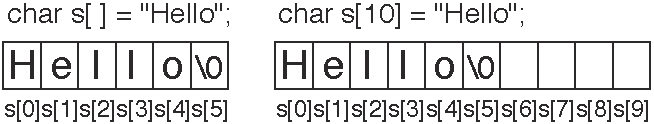
\includegraphics{hello.pdf}}
\end{center}
\end{figure}

\subsection{標準入力(1) : {\tt gets}関数}
例\ref{ex:gets}を作成しコンパイルしてみよう(コンパイラによっては、「\verb|gets| は危険だ」と警告が出るかもしれないが、実行ファイルはちゃんとできているはずである)。これを実行すると、\verb|Input:| と表示され入力を促される。ここで、\verb|uni|などと入力すると、\verb|uni|と表示されてプログラムが終了する。この場合、\verb|gets|という関数によって入力された文字列が \verb|str| にコピーされる。注意すべきことは、\verb|str| が \verb|str[20]| と宣言されているので入力すべき文字列は19文字以内に限られるということである。しかし実際には、ユーザーは20字以上入力することができる。その場合、はみ出た文字は用意された領域の外に書き込まれる。もしそこが、別の変数用に使われていたら? これはとても危険なことである。\verb|gets|を使う場合は注意が必要である。
\begin{reidai}\label{ex:gets}
\begin{verbatim}
#include <stdio.h>
int main() {
  char str[20];
  printf("Input: ");
  gets(str);
  printf("%s\n", str);
  return 0;
}
\end{verbatim}
\end{reidai}

\subsection{標準入力(2) : {\tt scanf}関数}
例\ref{ex:gets}ではたとえ数字(19桁以下)を入力してもそれは文字列として扱われるため、数字として足し算などに用いるためには \verb|atoi|などの関数を用いる必要がある。数字を入力してそのまま数字として扱う方法を例\ref{ex:scanf}に示す。この場合、\verb|scanf| という関数を用いている。(ソースコード中の \verb|&i| や \verb|&x| の \verb|&| は今は気にしなくて良い。)
\begin{reidai}\label{ex:scanf}
\begin{verbatim}
#include <stdio.h>
#include <string.h>
int main() {
  int i;
  double x;
  printf("Input(int): ");
  scanf("%d", &i);
  printf("%d\n", i);
  printf("Input(double): ");
  scanf("%lf", &x);
  printf("%lf\n", x);
  return 0;
}
\end{verbatim}
\end{reidai}

\begin{renshuu}\label{prob:4-1}
練習\ref{prob:2-2}で、標準入力から $n$ を決定し、その答えを表示するプログラムを書きなさい。
\end{renshuu}

\section{ポインタ}

ポインタの習得はC言語の習得の中でひとつの大きな壁である。はじめは訳がわからないかもしれないが、C言語の基本的な部分の1つなので、いろいろな例に触れて慣れてほしい。慣れが一番である。

\subsection{とりあえず(1)}

例\ref{ex:pointer1}を作成し実行してみよう。上手くいけば、``{\tt q is 200 and *p is 200.}''と表示されるはずである。この例で出てくる \verb|p| がポインタである。\verb|int| 型のポインタを宣言するには、
\begin{quote}
\begin{verbatim}
int *p;
\end{verbatim}
\end{quote}
のように\verb|*|をつけて宣言する。そして、\verb|p| が \verb|int| のポインタで、\verb|*p| が \verb|int| になる。人によっては、
\begin{quote}
\begin{verbatim}
int* p;
\end{verbatim}
\end{quote}
と宣言したほうがイメージしやすいかもしれない。つまり、\verb|p| は \verb|int*| 型(\verb|int| のポインタ)ということである。(しかし、2個以上のポインタを宣言するためには、\verb|int *p, *q;| としなければならない。\verb|int* p, q;| とすると意味が変わってしまう。)

\verb|p| という \verb|int| 型のポインタは、\verb|int| 型の変数のアドレスを指し示す働きをする。アドレスとは大雑把にいえば、次のようなものである。例\ref{ex:pointer1}の \verb|int q; q = 200;| の \verb|q| に格納されている200はコンピュータのメモリーのどこかに電気的に存在するはずである。その物の場所を示すものがアドレスである。メモリー上の住所である。したがって、例\ref{ex:pointer1}では \verb|p = &q;| の文によって、\verb|p| は \verb|q| を指し示すことになる。(\verb|&q| は \verb|q| のアドレスを表す。) これにより、\verb|q| は \verb|q| 自身だけでなく、\verb|p| というポインタによってもアクセスすることができるようになる。
\begin{reidai}\label{ex:pointer1}
\begin{verbatim}
#include <stdio.h>
int main() {
  int *p;
  int q;
  q = 200;
  p = &q;
  printf("q is %d and *p is %d.\n", q, *p);
  return 0;
}
\end{verbatim}
\end{reidai}
\begin{figure}[H]
\begin{center}
\resizebox{0.50\textwidth}{!}{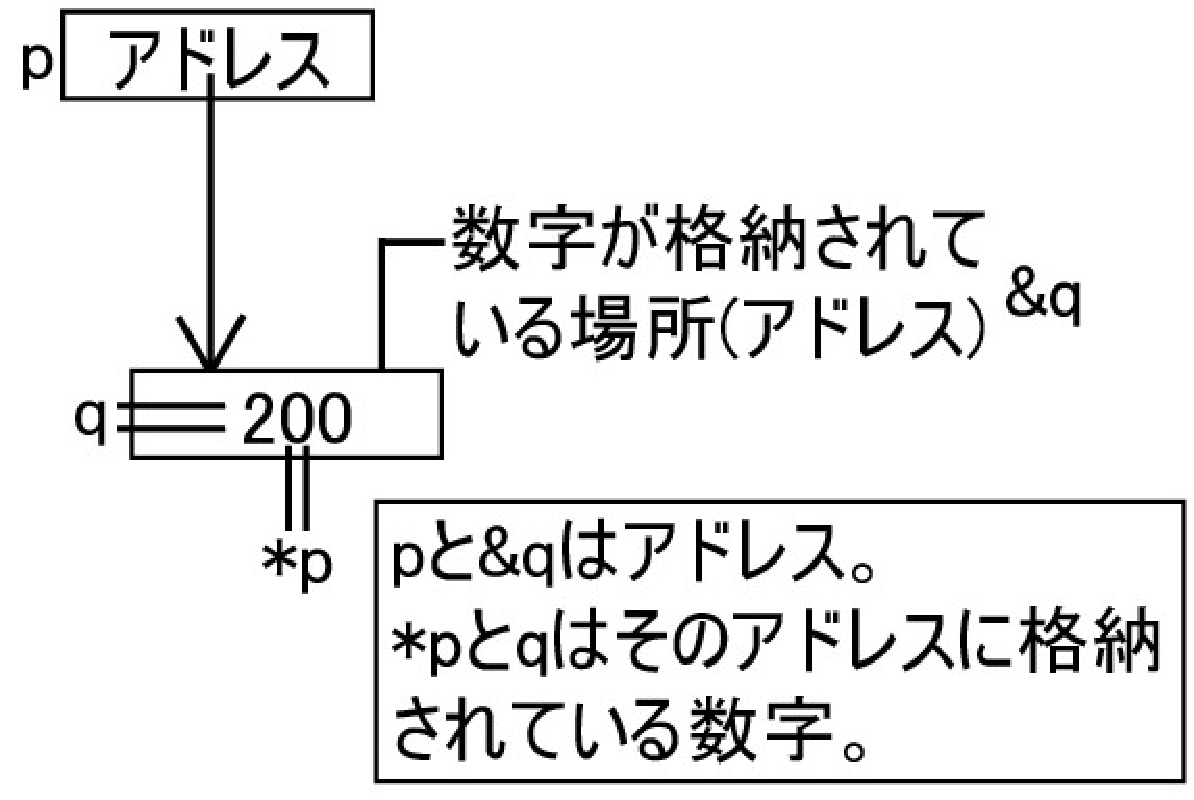
\includegraphics{pointer.pdf}}
\end{center}
\end{figure}

\subsection{とりあえず(2)}
では、もう1つ例を示そう。例\ref{ex:pointer2}では、\verb|p = &q;| により \verb|p| というポインタで \verb|q| にアクセスできる。ここでは、\verb|q| に値を代入するかわりに、\verb|*p|を用いて値を代入している。\verb|p|はポインタで、\verb|*p| は \verb|p| が示しているアドレスにある値そのものである。
実行結果は、``{\tt q is 300 and *p is 300.}''となる。
\begin{reidai}\label{ex:pointer2}
\begin{verbatim}
#include <stdio.h>
int main() {
  int *p;
  int q;
  p = &q;
  *p = 300;
  printf("q is %d and *p is %d.\n", q, *p);
  return 0;
}
\end{verbatim}
\end{reidai} \noindent
記号{\tt *}, {\tt \&}などの意味と役割をもう一度復習しておこう。
\begin{quote}
\begin{verbatim}
int *p;
int q;
\end{verbatim}
\end{quote}
の時、
\begin{table}[H]
\begin{center}
\begin{tabular}{ll}
  \verb|p|  &ポインタ (つまりどこかのアドレス)\\
  \verb|*p| &実体\\
  \verb|q|  &実体\\
  \verb|&q| &\verb|q| のアドレス
\end{tabular}
\end{center}
\end{table} \noindent
注意すべきことは、例\ref{ex:pointer1}や例\ref{ex:pointer2}で \verb|p = &q;| がない場合は \verb|p| がどこを指しているか未定義であるということだ。したがって、\verb|*p = 300;| や \verb|printf| 内で \verb|*p| を表示させるのは危険である。何が起こるか分からない。

この節では、静的に宣言された変数を指すためにポインタを用いてきたが、より高度な使い方については\ref{sec:clang:malloc}節で紹介する。

\subsection{ポインタと配列}
\label{sec:C:pointer-array}
ポインタと配列には密接な関係がある。
\begin{quote}
\begin{verbatim}
int array[10];
\end{verbatim}
\end{quote}
と宣言した場合、\verb|array[0]| や \verb|array[5]| などで配列の要素にアクセスすることができた。実は、\verb|array| だけでも意味を持つ。\verb|array| は配列型 (\verb|int[10]| 型) の変数で、プログラムコード中に登場した時は、大抵の状況では、自動的に ``配列の先頭要素のアドレス''に暗黙的に変換されて解釈される。つまり、\verb|array| は \verb|array[0]| へのポインタとして解釈され、\verb|*array| は \verb|array[0]|を意味する。さらに、ポインタに整数を足すとその数だけ先の要素を指すようになる。例えば\verb|array+2|は\verb|array[2]| へのポインタであり、\verb|*(array+2)| は \verb|array[2]|と等価である。

では、例\ref{ex:pointer-array}を見てみよう。\verb|strlen| という関数は string.h 内で宣言されている文字列の長さを返す関数である。最初の \verb|for| 文は文字型の配列 \verb|str| の中身を順番に書き出している。次の \verb|for| 文がポイントである。まず、文字型のポインタ \verb|p| に文字型の配列 \verb|str| の先頭ポインタ \verb|str| を代入している。そして、文字型の実体である \verb|*p| が \verb|\0| でない場合はその \verb|*p| を表示し、ポインタ \verb|p| の指す部分をひとつ進めている。これを \verb|*p| が \verb|\0| になるまで繰り返すことで、最初の \verb|for| 文と同じ結果を表示している。
\begin{reidai}\label{ex:pointer-array}
\begin{verbatim}
#include <stdio.h>
#include <string.h>
int main() {
  char str[] = "ABCDE";
  int num = strlen(str);
  int i;
  for (i = 0; i < num; ++i) {
    printf("%c", str[i]);
  }
  printf("\n");
  char *p;
  for (p = str; *p != '\0'; ++p) {
    printf("%c", *p);
  }
  printf("\n");
  return 0;
}
\end{verbatim}
\end{reidai}

\begin{renshuu}\label{prob:5-1}
次のプログラムの \verb|printf| の部分を配列ではなく、ポインタを使ったものに書き換えなさい。(\verb|array| を使っても、あるいは、\verb|int *p;| を加えてもよい。)

\begin{quote}
\begin{verbatim}
#include <stdio.h>
int main() {
  int i;
  int array[10];
  for (i = 0; i < 10; ++i) {
    array[i] = i*i;
  }
  for (i = 0; i < 10; ++i) {
    printf("array[%d] = %d\n", i, array[i]);
  }
  return 0;
}
\end{verbatim}
\end{quote}
\end{renshuu}

\section{関数}
\label{sec:C:function}

\ref{sec:C:basic}節でC言語の基本構造を説明したが、\verb|main(){...}| だけでプログラムを書くことはほとんどない。大きなプログラムになればなるほど関数化を行い、役割分担をはっきりさせるのがよい。

\subsection{あまり良くない例}
例\ref{ex:non-function}は円の面積の計算するために直接その公式を書いている。しかし、何度も何度も円の面積を計算したいとき、半径を入力すれば面積が返ってくるような関数があれば非常に便利である。
\begin{reidai}\label{ex:non-function}
\begin{verbatim}
#include <math.h>
#include <stdio.h>
int main() {
  double radius = 2.0;
  double area = radius * radius * M_PI;
  printf("Radius: %lf, Area: %lf\n", radius, area);
  return 0;
}
\end{verbatim}
\end{reidai}

\subsection{関数化}
では、例\ref{ex:non-function}を例\ref{ex:function1}のように変更してみよう。このような小さなプログラムでは関数化の効力は乏しいが、大きくなればなるほど、また複雑になればなるほど、その効力は絶大になる。例\ref{ex:function1}では、\verb|circle_area| という関数が定義されている。この関数は、double型の値を引数として受け取り、面積を計算してその値を戻り値にしている。関数は使う前に宣言する必要がある。したがって、\verb|circle_area| 関数を \verb|main| の後や他のファイルに書く場合は、例\ref{ex:function2}のように使う前に宣言だけ行っておく必要がある。
\begin{reidai}\label{ex:function1}
\begin{verbatim}
#include <math.h>
#include <stdio.h>
double circle_area(double r) {
  return r*r*M_PI;
}

int main() {
  double radius = 2.0;
  double area = circle_area(radius);
  printf("Radius: %lf, Area: %lf\n", radius, area);
  return 0;
}
\end{verbatim}
\end{reidai}
\begin{reidai}\label{ex:function2}
\begin{verbatim}
#include <math.h>
#include <stdio.h>
double circle_area(double);

int main() {
  double radius = 2.0;
  double area = circle_area(radius);
  printf("Radius: %lf, Area: %lf\n", radius, area);
  return 0;
} 

double circle_area(double r) {
  return r*r*M_PI;
}
\end{verbatim}
\end{reidai}

\subsection{ポインタを引数にする関数}

例\ref{ex:function1}では関数の返り値が面積の1つだけであった。しかし、例えば割り算で商と余りを返したい場合、例\ref{ex:function1}のような関数ではうまく実現できない。なぜなら、戻り値は1個しか指定できないからである。これを解決するには、ポインタを引数とする関数を作る必要がある。答えを入れる箱をあらかじめ準備しておき、それを関数の引数にポインタとして渡し、関数内でそこに答えを入れてもらって、関数の外で受け取るという方法を用いる。重要な点は、ポインタでなければ関数内で代入した値を関数の外で使うことはできないということである。

例\ref{ex:function-pointer}では、まず{\tt main}で答えを入れてもらうための \verb|shou| と \verb|amari| という箱(変数)を準備している。次に、そのポインタ(アドレス)を関数\verb|division|に渡している。そして、\verb|division|内で答えを代入してもらい、関数の外で\verb|printf|を用いて答えを表示している。\verb|division| という関数の先頭にある\verb|void|という型は(返り値の形では)何も返さないことを示すためのものである。
\begin{reidai}\label{ex:function-pointer}
\begin{verbatim}
#include <stdio.h>
void division(int divident, int divisor, int *quotient, int *residual) {
  *quotient = divident / divisor;
  *residual = divident % divisor;
}

int main() {
  int josuu = 3;
  int hi_josuu = 13;
  int shou, amari;
  division(hi_josuu, josuu, &shou, &amari);
  printf("%d / %d = %d ... %d\n", hi_josuu, josuu, shou, amari);
  return 0;
}
\end{verbatim}
\end{reidai} \noindent
ポインタを使う理由がはっきりと分からない場合は、例\ref{ex:function-non-pointer}を作って実行してみてほしい。間違った答えが表示されるだろう。なぜなら、この場合 \verb|division| という関数では、\verb|quotient|と\verb|residual|という二つの一時変数が生成され、それらに計算結果が代入されるからである。それらの一時変数は関数の処理が終了すると同時に破棄され、値は \verb|main| の中の \verb|shou| と \verb|amari| には引き継がれない。関数に外部から値を渡すだけであれば、例\ref{ex:function-non-pointer}のような引数の宣言方法で良い(「値渡し」とよぶ)が、内での計算結果を関数の外で使いたい場合は、ポインタを使って変数のアドレスを渡す(「ポインタ渡し」とよぶ)必要がある。
\begin{reidai}\label{ex:function-non-pointer}
\begin{verbatim}
#include <stdio.h>
void division(int divident, int divisor, int quotient, int residual) {
  quotient = divident / divisor;
  residual = divident % divisor;
}

int main() {
  int josuu = 3;
  int hi_josuu = 13;
  int shou, amari;
  division(hi_josuu, josuu, shou, amari);
  printf("%d / %d = %d ... %d\n", hi_josuu, josuu, shou, amari);
  return 0;
}
\end{verbatim}
\end{reidai}

\subsection {Fortranの関数や手続きの利用}

LAPACK\footnote{行列の対角化、連立一次方程式の求解など線形計算を行うライブラリ。ほぼ全ての計算機で利用可能である。}などの多くのライブラリがFortranで書かれている。これらと同等の機能を持つ関数をCやC++で作ることもできるが、既に存在するのであればそちらを使った方が便利である。ここでは、C言語の中からFortranの関数や手続きを呼ぶ方法を簡単に紹介する。

Fortranの関数や手続きの名前をC言語から呼ぶためには、その名前をすべて小文字にして、最後に\_ (下線)を付けなければならない。また、関数などの引数の型も適切に読み変える必要がある。例えば、
\begin{reidai}
\begin{verbatim}
      Real*8 CALC(I, X, Y)
      Interger*4 I
      Real*4 X
      Real*8 Y
\end{verbatim}
\end{reidai} \noindent
というFortranの関数が存在するとする。このときCでは次のように使う。
\begin{reidai}
\begin{verbatim}
extern double clac_(int*, float*, double*);

int main() {
  int i = 10;
  float x = 20.0;
  double y = 30.0;
  double ret = calc_(&i, &x, &y);
  retrun 0;
}
\end{verbatim}
\end{reidai} \noindent
全ての引数をポインタ渡しとしなければならないことに特に注意せよ。コンパイルはCとFortranで別々に行い、最後にリンクすればよい。

\section{構造体}
データ構造を取り扱うためには構造体を用いる。

例\ref{ex:struct1}を見てほしい。個人のデータを取り扱うために \verb|personal_data| という1つの箱を準備している。これが構造体である。もし構造体を使わなければ、同じ内容のプログラムを実現するためには複数の配列を準備する必要が出てくる。これは見た目にも格好悪いし、拡張性も乏しく複雑になる。例\ref{ex:struct1}では、\verb|struct personal_data pdata;| で \verb|pdata| を構造体とし宣言している。少し分かりにくいかもしれないが、\verb|int n;|と比べてみると、\verb|int| と ``\verb|struct personal_data|''が同じ立場であって、\verb|int| と ``\verb|struct|''が同じ立場というわけではないことに注意してほしい。\verb|int| という型はあらかじめC言語で決められた型なのに対し、構造体は自分が好きなように使いやすいように決めた型だと考えても構わない。つまり、``\verb|struct personal_data|''型というものを自分で作ったと考えるのである。そうすれば、\verb|struct personal_data pdata;| という使い方も理解できるはずである。

構造体内の各データには、ドット演算子 (\verb|.|) を使ってアクセスする。また、年齢を文字列 \verb|buffer[16]| として受け取っているため、\verb|atoi| 関数を用いて数字に変換している。\verb|atoi| は文字列を整数に変換する関数である。詳しくはコマンドラインで \verb|man atoi| としてみよ。
\begin{reidai}\label{ex:struct1}
\begin{verbatim}
#include <stdio.h>
#include <stdlib.h>
struct personal_data {
  char family_name[16];
  char given_name[16];
  int age;
};

int main() {
  struct personal_data pdata;
  char buffer[16];
  printf("Input family name: ");
  gets(pdata.family_name);
  printf("Input given name: ");
  gets(pdata.given_name);
  printf("Input age: ");
  gets(buffer);
  pdata.age = atoi(buffer);
  printf("Family Name = %s\n", pdata.family_name);
  printf("Given  Name = %s\n", pdata.given_name);
  printf("Age         = %d\n", pdata.age);
  return 0;
}
\end{verbatim}
\end{reidai} \noindent
構造体を指すポインタの場合は、次の例\ref{ex:struct2}のように、アロー演算子 (\verb|->|) でその構造体の要素にアクセスすることができる。例題中の\verb|qdata->p[0]|は\verb|(*qdata).p[0]|と等価である。ちなみに、この例の構造体は粒子の質量と運動量を格納している。
\begin{reidai}\label{ex:struct2}
\begin{verbatim}
#include <stdio.h>
struct particle_data {
  double mass;
  double p[3]; /* Momentum */
};

int main() {
  struct particle_data pdata;
  struct particle_data *qdata;
  pdata.mass = 0.14;
  pdata.p[0] = 1.2;
  pdata.p[1] = 1.3;
  pdata.p[2] = 1.4;
  qdata = &pdata;
  printf("Mass = %lf\n", qdata->mass);
  printf("Momentum = (%lf, %lf, %lf)\n", qdata->p[0], qdata->p[1], qdata->p[2]);
  return 0;
}
\end{verbatim}
\end{reidai}
\begin{renshuu}\label{prob:7-1}
``月'', ``日'', ``1月1日からの日数(うるう年ではない)''を構成要素とする構造体を作って、``月'' と ``日''を標準入力から入力すれば、自動的に ``1月1日からの日数''の部分を埋め、最後にそれを表示して終了するプログラムを書きなさい。
\end{renshuu}

\section{ファイルの取り扱い}

ファイルから数字を読みこんだり、ファイルに結果を書き込んだりするプログラムを紹介する。ここで挙げた例だけでも基本的なことはできるはずである。より詳しく知りたい場合は参考書などを参照してほしい。

\subsection{ファイルから数字の読み込み}

例\ref{ex:file-read1}がファイルから数字を読み込むときの雛型となる。まず、\verb|FILE *fp;| でファイルを取り扱うための構造体を宣言する。\verb|char *filename|の部分でファイル名を宣言する。そして、\verb|fopen|でファイルを開く。(\verb|"r"| はread (読み取り専用)でファイルを開くことを示す。) \verb|if(fp==NULL){}| の部分はエラーが起こったときに処理され、プログラムを強制終了させる。\verb|fscanf|で順番にファイルに書かれている数字を\verb|double|型で読み取っている。\verb|fscanf|の使い方は、
\begin{quote}
\begin{verbatim}
fscanf(ファイル構造体のポインタ, "フォーマット", &変数1, &変数2, ......);
\end{verbatim}
\end{quote}
で、ファイル構造体のポインタ部分以外は \verb|scanf| と同じである。そして、最後に \verb|fclose(fp);| でファイルを閉じている。
\begin{reidai}\label{ex:file-read1}
\begin{verbatim}
#include <stdio.h>
#include <stdlib.h>
double product(double x1, double y1, double x2, double y2) {
  return x1*y1 + x2*y2;
}

int main() {
  FILE *fp;
  char *filename = "vectors.txt";
  double x1,y1,x2,y2,p;
  fp = fopen(filename, "r");
  if (fp == NULL) {
    printf("Can't open file %s\n", filename);
    exit( 1 );
  }
  /* read first line */
  fscanf(fp, "%lf %lf\n", &x1, &y1);
  /* read second line */
  fscanf(fp, "%lf %lf\n", &x2, &y2);
  fclose(fp);
  p = product(x1, y1, x2, y2);
  printf("Product of (%lf,%lf) and (%lf,%lf) is %lf\n", x1, y1, x2, y2, p);
  return 0;
}
\end{verbatim}
\end{reidai} \noindent
例\ref{ex:file-read1}を実行するためには、{\tt vectors.txt}というファイル名で以下のような内容の入力ファイルも作っておく必要がある。
\begin{quote}
\begin{verbatim}
 1.0    2.0
-1.5    3.5
\end{verbatim}
\end{quote}
例\ref{ex:file-read1}のデータを読み込む部分を、例\ref{ex:file-read2}のように \verb|while| を使って書き直してみよう。こちらの方がファイルに存在するデータを最後まで読み取るという点で、より汎用性が高い。\verb|fscanf|はデータの読み込みに失敗すると\verb|EOF|を返すので、\verb|EOF|が返ってくるまで読み込みを繰り返している。
\begin{reidai}\label{ex:file-read2}
\begin{verbatim}
#include <stdio.h>
#include <stdlib.h>
#define N_DATA 100
int main() {
  FILE *fp;
  char *filename = "vectors.txt";
  double x[N_DATA][2];
  int index = 0;
  fp = fopen(filename, "r");
  if (fp==NULL) {
    printf("Can't open file %s\n", filename);
    exit(1);
  }
  /* read data */
  while (fscanf(fp, "%lf %lf\n", &x[index][0], &x[index][1]) != EOF) {
    printf("Data %d : (%lf, %lf)\n", index, x[index][0],x[index][1]);
    ++index;
  }
  fclose(fp);
  return 0;
}
\end{verbatim}
\end{reidai}

\subsection{ファイルへの数字の書き出し}

例\ref{ex:file-write}がファイルへ数字を書き出すときの雛型である。ファイルを開くところまでは例\ref{ex:file-read1}とはほぼ同じで、違う点は \verb|fopen| の第2引数が \verb|"r"| ではなく \verb|"w"| (書きこみ)である点である。また、書き出すときには \verb|fprintf| という関数を使っている。\verb|fprintf| の使い方は、
\begin{quote}
\begin{verbatim}
fprintf(ファイル構造体のポインタ, "フォーマット", 変数1, 変数2, ......);
\end{verbatim}
\end{quote}
で、ファイル構造体のポインタ部分以外は \verb|printf| と同じである。最後に、\verb|fclose(fp);| でファイルを閉じる。
\begin{reidai}\label{ex:file-write}
\begin{verbatim}
#include <stdio.h>
#include <stdlib.h>
#include <math.h>
double circle_area(double r) {
  return r*r*M_PI;
}

int main() {
  FILE *fp;
  char *filename = "circle_area.txt";
  double radius;
  int i;
  fp = fopen(filename, "w");
  if (fp == NULL) {
    printf("Can't open file %s\n", filename);
    exit(1);
  }
  for(i = 1; i <= 10; ++i) {
    radius = i * 1.0;
    double area = circle_area(radius);
    fprintf(fp, "%lf -> %lf\n", radius, area);
  }
  fclose(fp);
  return 0;
}
\end{verbatim}
\end{reidai}

\section{その他の制御文}

 {\tt for}, {\tt while}以外の制御文の書式を紹介する。

\subsection{{\tt switch}-{\tt case}文}

1の場合にはAを、2の場合にはBを、3の場合にはCを、という風に条件分岐をしたい場合に、\verb|switch|-\verb|case|文を用いる。
\begin{reidai}\label{ex:case}
\begin{verbatim}
#include <stdio.h>
#include <string.h>
int main() {
  int i;
  printf("Input(int): ");
  scanf("%d", &i);
  printf("%d / 3 no amari ha ", i);
  switch (i%3) {
    case 1:
      printf("1 desu.\n");
      break;
    case 2:
      printf("2 desu.\n");
      break;
    default:
      printf("0 desu.\n");
  }
  return 0;
}
\end{verbatim}
\end{reidai} \noindent
\verb|i%3|の結果が1であれば、\verb|case 1:| 以下の部分から実行する。\verb|i%3|の結果が2であれば、\verb|case 2:| 以下の部分から実行する。\verb|i%3|の結果が1でも2でもない場合、つまり、0の場合は、\verb|default:| 以下の部分から実行する。もちろん、\verb|case 0:| を作っても構わない。注意としては、もし例\ref{ex:case}の \verb|switch|-\verb|case| 文中に \verb|break;| がないと、\verb|case 1:| の場合は \verb|case 2:| の部分も \verb|default:| の部分も実行してしまうことである。つまり、\verb|case 1:| 以下の部分から下の部分をすべて実行するというこである。したがって、\verb|case 2:| の直前で抜けるためには \verb|break;| が必要となる。実際に \verb|break;| を削除して試してみよう。この場合は常に \verb|...0 desu.| が表示されるはずである。\verb|switch|-\verb|case| 文を簡単にまとめると、次のようになる。
\begin{quote}
\begin{verbatim}
switch (X) {
  case A:  ブロック1
  case B:  ブロック2
  case C:  ブロック3
  default: ブロック4
}
\end{verbatim}
\end{quote}
\verb|X|が\verb|A|ならば、ブロック1以下すべてを実行する。\verb|X|が\verb|B|ならば、ブロック2以下をすべて実行する。\verb|X|が\verb|C|ならばブロック3以下をすべて実行する。\verb|X|が\verb|A|でも\verb|B|でも\verb|C|でもない場合は、ブロック4を実行する。

\subsection{{\tt do}-{\tt while}文}

\verb|while| 文と同様に、ある条件が満たされている場合に繰り返しを行うために \verb|do|-\verb|while| 文を使う。\verb|while| 文と違う点は、条件の判定する``タイミング''である。\verb|while| 文の場合は、まず条件を判定し、満足していれば\verb|while| 内を実行するが、\verb|do|-\verb|while| 文の場合は、まず\verb|do|-\verb|while| 内を実行してから条件を判定する。したがって、\verb|while| 文の場合は \verb|while| 内を1度も実行しない場合があるが、\verb|do|-\verb|while| 文の場合は必ず1度は \verb|do|-\verb|while| 内を実行する。
\begin{reidai}\label{ex:do-while}
\begin{verbatim}
#include <stdio.h>
int main() {
  int i = 100;
  int sum = 0;
  do {
    sum += i;
    --i;
  } while (i != 0);
  printf("sum of integers from 100 to 1 is %d\n", sum);
  return 0;
}
\end{verbatim}
\end{reidai} \noindent
例\ref{ex:do-while}のように、\verb|while()| の後の \verb|;| を忘れないこと。
\verb|do|-\verb|while| 文の基本的な動作は次のようになる。
\begin{quote}
\begin{verbatim}
do {
  ブロック
} while (A);
\end{verbatim}
\end{quote}
まずブロックを実行し、次にAをチェックして正しいならば、再びブロックを実行する。そして、再びAをチェックして正しいならば、ブロックを実行する。したがって、Aが最初から間違いであってもブロックは必ず一度は実行される。

\section{コマンドライン引数の受け渡し}
{\tt main}文には、\verb|int main()| 以外に、\verb|int main(int, char**)|, あるいは \verb|int main(int, char*[])| という書き方がある。これらの書式を利用すれば、実行時に引数を与えてそれを利用することができる。つまり、今までは
\begin{commandline2}
\prompt \underline{./a.out}
\end{commandline2} \noindent
であったが、これを利用すれば、
\begin{commandline2}
\prompt \underline{./a.out input.data output.data}
\end{commandline2} \noindent
のように、ファイル名や数値などをコマンドライン引数としてプログラムに渡すことができる。

\subsection{ポインタ配列}

新しい\verb|main|関数の説明の前に、引数の受け渡しに使われているポインタ配列に関して説明しておこう。ポインタ配列は、名前通り、ポインタを要素とする配列(\verb|char*[]|)である。配列はポインタを使ってアクセス可能なので、``ポインタのポインタ'' (\verb|char**|)と同様に使うことができる。
\begin{reidai}\label{ex:pointers-array}
\begin{verbatim}
#include <stdio.h>
int main() {
  int i;
  char *name0 = "Alice";
  char *name1 = "Bob";
  char *name2 = "Claire";
  char *name3 = "David";
  char *name[4];
  name[0] = name0;
  name[1] = name1;
  name[2] = name2;
  name[3] = name3; /* A */
  for (i = 0; i < 4; ++i) { /* B */
    printf("Name%d : %s\n", i, name[i]);
  }
  for (i = 0; i < 4; ++i) { /* C */
    printf("Name%d : %c, %s\n", i, **(name+i), *(name+i));
  }
  return 0;
}
\end{verbatim}
\end{reidai} \noindent
例\ref{ex:pointers-array}の結果は以下のようになる。
\begin{quote}
\begin{verbatim}
Name0 : Alice
Name1 : Bob
Name2 : Claire
Name3 : David
Name0 : A, Alice
Name1 : B, Bob
Name2 : C, Claire
Name3 : D, David
\end{verbatim}
\end{quote}
まず、\verb|name[0]| の型は \verb|char*| なので、\verb|name0| の値等を代入することができる。Aの時点で、\verb|name| というポインタ配列の各要素にアドレスの代入したことになる。つまり、
\begin{quote}
\begin{verbatim}
name[0] = "Alice"という文字列の先頭アドレス
name[1] = "Bob"という文字列の先頭アドレス
name[2] = "Claire"という文字列の先頭アドレス
name[3] = "David"という文字列の先頭アドレス
\end{verbatim}
\end{quote}
となっている。したがって、Bの \verb|for| 文では、\verb|printf| に文字列の先頭アドレスを渡すことで、名前を表示することができる。次に、Cの \verb|for| 文であるが、これは若干混乱を招くが、次が理解出来れば、何とかクリアできるだろう。
\begin{center}
\begin{tabular}{r@{ = }c@{ = }l}
\verb|name|   & 文字へのポインタのポインタ & \verb|char**| 型\\
\verb|*name|  & 文字へのポインタ           & \verb|char*| 型\\
\verb|**name| & 文字                       & \verb|char| 型 (※ 文字列ではなく文字)
\end{tabular}
\end{center}
\verb|printf| は \verb|%s| で文字列の先頭アドレス、つまり、\verb|char*| を受け取り、\verb|%c| で文字型そのもの、つまり、\verb|char| を受け取る。また、\verb|name+i| という書き方は、例えば、\verb|name+1| の場合なら、\verb|name| が \verb|name[0]| なので、\verb|name+1| は \verb|name[1]| である。

\subsection{新しい{\tt main}関数}

例\ref{ex:new-main}がコマンドライン引数を受け取ることのできる \verb|main|関数の例である。{\tt int main(int argc, char* argv[])}は、{\tt int main(int argc, char** argv)}と書いても同じである。好きなほうを使えばよい。
また、伝統的に \verb|argc| と \verb|argv| という名前を使っているが、他の変数名でも構わない。
\begin{reidai}\label{ex:new-main}
\begin{verbatim}
#include <stdio.h>
#include <stdlib.h>
int main(int argc, char* argv[]) {
  FILE *fp;
  char *InputFileName;
  char *OutputFileName;
  int counter = 0;
  double x,y;
  double sumX = 0.0, sumY = 0.0;
  if (argc != 3) { /* A */
    printf("Usage: sumXY InputFile OutputFile\n");
    exit(1);
  }
  InputFileName = argv[1];
  OutputFileName = argv[2];
  /* input */
  fp = fopen(InputFileName, "r");
  if (fp==NULL) {
    printf("Can't open file %s\n", InputFileName);
    exit(1);
  }
  /* read data */
  while(fscanf(fp, "%lf %lf\n", &x, &y) != EOF) {
    sumX += x;
    sumY += y;
    ++counter;
  }
  fclose(fp);
  /* output */
  fp = fopen(OutputFileName, "w");
  if (fp == NULL) {
    printf("Can't open file %s\n", OutputFileName);
    exit(1);
  }
  /* write results */
  fprintf(fp, "Number of Data = %d\n", counter);
  fprintf(fp, "X Sum = %lf\n", sumX);
  fprintf(fp, "Y Sum = %lf\n", sumY);
  fclose(fp);
  return 0;
}
\end{verbatim}
\end{reidai} \noindent
例\ref{ex:new-main}を\ref{ex:new-main}cという名前で保存し、次のようにコンパイルする。
\begin{commandline2}
\prompt \underline{gcc -o sumXY \ref{ex:new-main}c}
\end{commandline2} \noindent
\verb|sumXY|は例\ref{ex:new-main}のAの部分の\verb|printf|のメッセージに合わせてある。次のように実行してみよう。
\begin{commandline2}
\prompt \underline{./sumXY}\\
Usage: sumXY InputFile OutputFile
\end{commandline2} \noindent
{\tt InputFile}, {\tt OutputFile}の二つのコマンドライン引数が必要であるという警告が表示される。例\ref{ex:new-main}のAの部分を変更することで、警告メッセージは変更することができる。次のように実行しても同じメッセージが出力されるはずである。
\begin{commandline2}
\prompt \underline{./sumXY input.dat}
\end{commandline2} \noindent
\begin{commandline2}
\prompt \underline{./sumXY input.dat output.dat 10}
\end{commandline2} \noindent
一番目の例は引数が足りず、二番目の例は引数が多すぎる。例\ref{ex:new-main}では \verb|argc| が3以外ならエラーメッセージを表示するようにしてあるので、
\begin{commandline2}
\prompt \underline{./sumXY input.dat output.dat 10}
\end{commandline2} \noindent
は3個の引数だからエラーが出るのはおかしい、と考えるかもしれない。しかし、これは正しい動作である。なぜなら、引数としてプログラム名(\verb|./sumXY|)も1個と数えられるからである\footnote{{\tt argv[0]}を用いると、例\ref{ex:new-main}のAのエラーメッセージは {\tt printf("Usage: \%s InputFile OutputFile\textbackslash n", argv[0]);}と書くことができる。このようにしておくと、プログラム名をあらかじめソースコードに明示的に書き込む(「ハードコーディング」とよぶ)必要がなくなる。}。つまり、二番目の例では、{\tt argc}の値は4であり、{\tt argv}の中身は
\begin{quote}
\begin{verbatim}
argv[0] = "./sumXY"の先頭アドレス
argv[1] = "input.dat"の先頭アドレス
argv[2] = "output.dat"の先頭アドレス
argv[3] = "10"の先頭アドレス
\end{verbatim}
\end{quote}
となっている。

最後に、1行に2個の数字で10行程度書いた{\tt input.dat}を作成し、次のように実行してみよう。{\tt output.dat}に結果が書き込まれているはずである。
\begin{commandline2}
\prompt \underline{./sumXY input.dat output.dat}
\end{commandline2}

\section{動的な配列の確保: {\tt malloc}と{\tt free}}
\label{sec:clang:malloc}

これまで、ポインタはあらかじめ確保した領域に対してのみ使ってきた。しかし、実行時に、入力値あるいは計算結果を反映して、50個のデータを取り扱いたいときもあれば、100個のデータを取り扱いたいときもある。もちろん、配列を利用してあらかじめ十分な大きさの領域(いまの場合は100個以上の数)を確保しておけばよいかもしれないが、平均的に10個ぐらいしか利用しないのに、たまに100個の場合があるからといって常に100個分の領域を確保しておくことは、無駄のように思える。これを回避するために、動的に、つまり、実行時に領域を確保する手段がある。それが、\verb|malloc| ({\bf m}emory {\bf alloc}cationの略)である。

\subsection{{\tt malloc}の使い方}

例\ref{ex:malloc}に\verb|malloc|の使い方の雛型を示す\footnote{簡単のため、コマンドライン引数のチェックは行っていない。実際のプログラムでは、配列を確保する前に確保しようとしているサイズを確認すべきである。}。\verb|malloc|は領域が確保できた場合はその領域の先頭アドレスを返すが、領域が確保できなかった場合は\verb|NULL|を返す。\verb|NULL|の場合は、何らかのエラー処理を行う必要がある。例\ref{ex:malloc}では、プログラムを強制的に終了している。\verb|sizeof|関数は型の大きさ(バイト数)を調べる関数である。この場合は\verb|int|の大きさ(通常4)を調べている。\verb|double|を大きさを調べたい場合は\verb|sizeof(double)|のように使う。例\ref{ex:malloc}では、\verb|int| の領域を \verb|n_element| 個分確保したいので、\verb|sizeof(int)*n_element|を\verb|malloc|に与えている。
\begin{reidai}\label{ex:malloc}
\begin{verbatim}
#include <stdio.h>
#include <stdlib.h>
int main(int argc, char* argv[]) {
  int* array;
  int n_element = atoi(argv[1]);
  if ((array = malloc(sizeof(int)*n_element)) == NULL) {
    printf("Can't allocate memory.\n");
    exit(1);
  }
  int i;
  for (i = 0; i < n_element; ++i) {
    array[i] = i*i;
  }
  for (i = 0; i < n_element; ++i) {
    printf("array[%d] = %d\n", i, array[i]);
  }
  return 0;
}
\end{verbatim}
\end{reidai} \noindent
なお、コンパイル時に、{\tt malloc}の部分で``型の不整合'' という警告が出る場合は、つぎのように明示的に型を変換すればよい。
\begin{quote}
\begin{verbatim}
array = (int*)malloc(sizeof(int)*n_element)
\end{verbatim}
\end{quote}
これをキャスト(型変換)という。

\subsection{{\tt free}の使い方}

例\ref{ex:malloc}には(引数の数のチェック以外にも)適切でない部分がある。\verb|malloc|で確保した領域を解放していない点である。確保した領域を解放するためには、\verb|free|という関数を使う\footnote{例\ref{ex:malloc}のようにプログラムがすぐに終了してしまう場合には、{\tt free}は必要ないと主張する人がいるかもしれない。その主張も確かに間違っている訳ではないが、本当に必要なときに忘れないために普段から書く癖をつけるべきである。}。
具体的には、例\ref{ex:malloc}の \verb|return 0;| の前に
\begin{verbatim}
     free(array);
\end{verbatim}
と1行書けば良い。

次に、例\ref{ex:malloc}を若干変更し、\verb|free|が重要となる例を考えよう。
\begin{reidai}\label{ex:malloc-free}
\begin{verbatim}
#include <stdio.h>
#include <stdlib.h>
int main(int argc, char* argv[]) {
  int* array;
  int n_element = atoi(argv[1]);
  int i, j;
  for (j = 0; j < 3; ++j) {
    if ((array = malloc(sizeof(int)*n_element) == NULL) {
      printf("Can't allocate memory.\n");
      exit(1);
    }
    for (i = 0; i < n_element; ++i) {
      switch (j) {
        case 0:
          array[i] = i;
          break;
        case 1:
          array[i] = i*i;
          break;
        default:
          array[i] = i*i*i;
      }
    }
    for (i = 0; i < n_element; ++i) {
      printf("array[%d] = %d\n", i, array[i]);
    }
    free(array);
  }
  return 0;
}
\end{verbatim}
\end{reidai} \noindent
もし仮に\verb|free| がない場合、\verb|j=1| のとき、\verb|malloc| に成功すると \verb|array| は新しく確保された領域の先頭アドレスを持つ。この時、\verb|j=0|で確保した領域はどうなったのだろうか? その領域は、このプログラム自身が確保した領域として、このプログラムが終了するまで解放されない。しかも、\verb|array| はすでに \verb|j=0| のときに確保した領域を忘れているので、このプログラムからもその領域に適切にアクセスすることはできない。つまり、\verb|j=0| のときの領域はこのプログラムが持っているが、使うことができない領域として存在し続けることになる\footnote{これを「メモリリーク」と呼ぶ}。これは非常に無駄なことである。これを回避するためにも、使わなくなった領域は \verb|free| することが重要である。もちろん、最近の計算機はメモリ(および、スワップ領域)をたくさん積んでいるので例\ref{ex:malloc-free}程度のプログラムなら\verb|free|がなくても平気で最後まで動くはずであるが、習慣として、\verb|malloc| した領域を使い終わったら必ず \verb|free| するのがよい。

\subsection{動的な二次元配列}

C言語において、二次元配列は 一元配列の先頭を指すポインタの配列として表すことができる。
すなわち、各行をそれぞれ一次元配列として考え、各行の先頭を指すポインタを別の一次元配列に格納しておけばよい。
この場合、後者の配列は要素がポインタ型の配列であるので、double型の二次元配列の場合には
\begin{quote}
\begin{verbatim}
double** matrix;
\end{verbatim}
\end{quote}
と宣言する必要がある。その後、各行に対応する一次元配列を \verb|malloc| する。
\begin{reidai}\label{ex:malloc-2dim}
\begin{verbatim}
#include <stdio.h>
#include <stdlib.h>
int main() {
  int m = 3;
  int n = 4;
  int i, j;
  double** matrix;
  if ((matrix = (double**)malloc(sizeof(double*)*m)) == NULL) {
    printf("Can't allocate memory.\n");
    exit(1);
  }
  for (i = 0; i < m; ++i) {
    if ((matrix[i] = (double*)malloc(sizeof(double)*n)) == NULL) {
      printf("Can't allocate memory.\n");
      exit(1);
    }
  }
  for (i = 0; i < m; ++i) {
    for (j = 0; j < n; ++j) {
      matrix[i][j] = (i+1)*(j+1);
    }
  }
  for (i = 0; i < m; ++i) {
    for (j = 0; j < n; ++j) {
      printf("matrix[%d][%d] = %lf\n", i, j, matrix[i][j]);
    }
  }
  for (i = 0; i < m; ++i) {
    free(matrix[i]);
  }
  free(matrix);
  return 0;
}
\end{verbatim}
\end{reidai} \noindent
この例では、$3 \times 4$の二次元配列(行列)を宣言している。まず、\verb|matrix| に長さ \verb|m| の一次元配列(要素はdoubleポインタ型)を確保する。さらに、各行を格納する長さ \verb|n| の一次元配列(要素はdouble型)を \verb|m| 個確保し、その先頭アドレスを \verb|matrix| に格納する。配列の$(i,j)$成分へのアクセスは、静的な二次元配列の場合と同じく \verb|matrix[i][j]| と書けばよい。\verb|matrix[i][j]| は \verb|*(*(matrix+i)+j)| と等価であることに注意せよ。\verb|*(matrix+i)| により $i$ 行目の先頭アドレスが得られ、それに $j$ を足したアドレスの中身を参照することで、$(i,j)$成分が得られる。確保したメモリの解放の際は、まず各行に対応する一次元配列を解放した後、最後にそれらの先頭先頭アドレスを格納していたdoubleポインタ型の一次元配列を解放する必要がある\footnote{解放の順番を間違うとエラーとなる。その理由を考えてみよ。}。

上記の方法で動的な二次元配列を取り扱えるようになるが、実際に行列としてLAPACKなどの数値計算ライブラリと組み合わせて使うには、2つの問題がある。1つ目は行列の要素の連続性の問題、2つ目は要素の並ぶ順番である。

LAPACKなどの数値計算ライブラリでは、行列の要素は全てメモリ上で連続であると仮定されている。しかし、上記の方法では、各行のデータは連続であるが、行と行の間が連続であるとは限らない。C言語では、連続した \verb|malloc| の呼び出しで連続したメモリ領域が割り当てられることは保証されていないためである。メモリ上で \verb|matrix[0][0]| の次には \verb|matrix[0][1]|、\verb|matrix[0][2]|、\verb|matrix[0][3]| と並ぶが、その次が \verb|matrix[1][0]| とは限らないのである。

この問題を解決するには、それぞれの行に対して \verb|malloc| を行うのではなく、一度に$m \times n$の長さのメモリを確保した上で、$n$要素毎の要素(各行の先頭に対応)のポインタををポインタ型配列に格納していけばよい。具体的には、コードを以下のように修正する。
\begin{reidai}\label{ex:malloc-2dim-continuous}
\begin{verbatim}
#include <stdio.h>
#include <stdlib.h>
int main() {
  int m = 3;
  int n = 4;
  int i, j;
  double** matrix;
  if ((matrix = (double**)malloc(sizeof(double*)*m)) == NULL) {
    printf("Can't allocate memory.\n");
    exit(1);
  }
  if ((matrix[0] = (double*)malloc(sizeof(double)*m*n)) == NULL) {
    printf("Can't allocate memory.\n");
    exit(1);
  }
  for (i = 1; i < m; ++i) {
    matrix[i] = matrix[i-1] + n;
  }
  for (i = 0; i < m; ++i) {
    for (j = 0; j < n; ++j) {
      matrix[i][j] = (i+1)*(j+1);
    }
  }
  for (i = 0; i < m; ++i) {
    for (j = 0; j < n; ++j) {
      printf("matrix[%d][%d] = %lf\n", i, j, matrix[i][j]);
    }
  }
  free(matrix[0]);
  free(matrix);
  return 0;
}
\end{verbatim}
\end{reidai} \noindent
修正前のコードと異なり、\verb|malloc| と \verb|free| は、それぞれ2回ずつしか呼び出されていないことに注意せよ。

次に、2つ目の問題、要素の並ぶ順番について考える。LAPACKなどの数値計算ライブラリは、Fortran言語を用いて書かれていることが多い。Fortran言語では、二次元配列(行列)の要素は各列の要素がメモリ上で連続して並ぶ。例えば、$3 \times 3$行列では、要素はメモリ上で、$(0,0) \rightarrow (1,0) \rightarrow (2,0) \rightarrow (0,1) \rightarrow (1,1) \rightarrow (2,1) \rightarrow (0,2) \rightarrow (1,2) \rightarrow (2,2)$ の順に配置される。これを「列優勢 (column-major)」と呼ぶ。一方、C言語では、メモリ上で \verb|A[0][0]| の次に配置されるのは \verb|A[0][1]| である。こちらは「行優勢 (row-major)」と呼ぶ。
\begin{figure}[H]
\begin{center}
\resizebox{0.60\textwidth}{!}{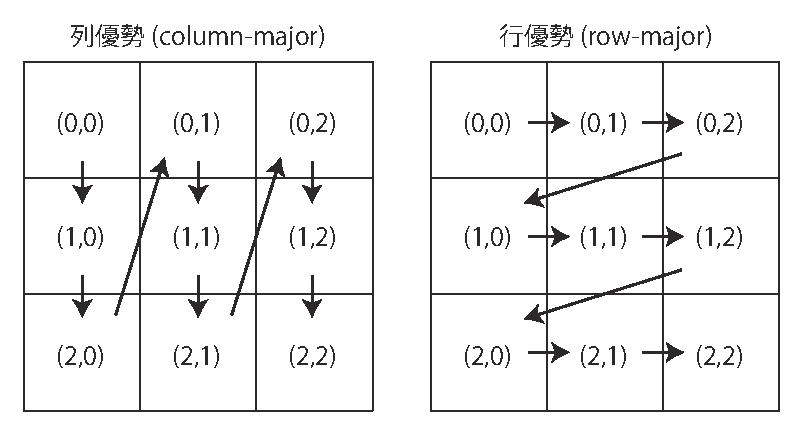
\includegraphics{major.pdf}}
\end{center}
\end{figure}
C言語上で行列の$(i,j)$成分を \verb|A[i][j]| に代入したもの(row-major)をLAPACKライブラリに渡すと、LAPACK側では要素がcolumn-majorで並んでいると解釈して計算を行う。すなわち、入力行列が転置されてしまう。また、計算結果もC言語から見ると転置された状態で返されることになってしまう。

これを防ぐには、行列の$(i,j)$成分を \verb|A[i][j]| ではなく \verb|A[j][i]| に格納するように決めてプログラムを書けばよいのだが、「常に順番を逆に書く」というのはプログラム作成時に混乱してしまう恐れがある。一つの解決方法は、C言語のマクロ機能を使い、プログラムの先頭で
\begin{quote}
\begin{verbatim}
#define mat_elem(mat, i, j) (mat)[(j)][(i)]
\end{verbatim}
\end{quote}
のように \verb|mat_elem| 関数を定義することである\footnote{一般的にC言語でのマクロの多用は勧められていないが、背に腹は代えられない。}。これにより、プログラム中で行列の$(i,j)$成分を \verb|mat_elem(A, i, j)| と書けるようになる。
\begin{reidai}\label{ex:malloc-2dim-column-major}
\begin{verbatim}
#include <stdio.h>
#include <stdlib.h>
#define mat_elem(mat, i, j) (mat)[(j)][(i)]
int main() {
  int m = 3;
  int n = 4;
  int i, j;
  double** matrix;
  if ((matrix = (double**)malloc(sizeof(double*)*n)) == NULL) {
    printf("Can't allocate memory.\n");
    exit(1);
  }
  if ((matrix[0] = (double*)malloc(sizeof(double)*m*n)) == NULL) {
    printf("Can't allocate memory.\n");
    exit(1);
  }
  for (i = 1; i < n; ++i) {
    matrix[i] = matrix[i-1] + m;
  }
  for (i = 0; i < m; ++i) {
    for (j = 0; j < n; ++j) {
      mat_elem(matrix, i, j) = (i+1)*(j+1);
    }
  }
  for (i = 0; i < m; ++i) {
    for (j = 0; j < n; ++j) {
      printf("matrix[%d][%d] = %lf\n", i, j, mat_elem(matrix, i, j));
    }
  }
  free(matrix[0]);
  free(matrix);
  return 0;
}
\end{verbatim}
\end{reidai} \noindent
プログラムの前半で、$m \times n$ではなく$n \times m$の二次元配列として配列を作成していることに注意せよ\footnote{列優勢(column-major)の二次元配列の確保や解放のための関数、および要素へのアクセス用のマクロ一式をまとめたものが、{\tt cmatrix.h} として{https://github.com/utphys-comp/cmatrix/}で公開されている。}。

\section{練習問題の解答例}

以下に練習問題の解答例を示す。さまざまなプログラムの書き方があるので、これらの解答例にこだわらないこと。全く分からない場合に参考にする程度が望ましい。
\begin{renshuu-answer}{prob:2-1}
\baselineskip=12pt
\begin{verbatim}
#include <stdio.h>
int main() {
  /* ax+b=0 */
  double a = 4.0;
  double b = 1.0;
  printf("ax+b=0\n");
  printf("  a = %lf\n", a);
  printf("  b = %lf\n\n", b);
  if (a == 0.) {
    if (b == 0.) {
      printf("  x = all\n");
    } else {
      printf("  x = nothing\n");
    }
  } else {
    printf("  x = %lf\n", -b/a);
  }
  return 0;
}
\end{verbatim}
\end{renshuu-answer}
\begin{renshuu-answer}{prob:2-2}
\baselineskip=12pt
\begin{verbatim}
#include <stdio.h>
#include <stdlib.h>
int main() {
  /* calculate "n!" */
  int n = 10;
  if (n < 1){
    printf("Can't calculate n!.\n");
    printf("n = %d\n",n);
    exit(1);
  }
  int ans = 1;
  int i;
  for (i = 1; i <= n; ++i) {
    ans *= i;
  }
  printf("%d! = %d\n",n,ans);
  return 0;
}
\end{verbatim}
\end{renshuu-answer}
\begin{renshuu-answer}{prob:2-2}
\baselineskip=12pt
\begin{verbatim}
#include <stdio.h>
#include <stdlib.h>
int main() {
  /* calculate "n!" */
  int n = 10;
  if (n < 1) {
    printf("Can't calculate n!.\n");
    printf("n = %d\n",n);
    exit(1);
  }
  int ans = 1;
  int i = 1;
  while (i <= n) {
    ans *= i;
    ++i;
  }
  printf("%d! = %d\n",n,ans);
  return 0;
}
\end{verbatim}
\end{renshuu-answer}
\begin{renshuu-answer}{prob:2-3}
\baselineskip=12pt
\begin{verbatim}
#include <stdio.h>
int main() {
  /* n madeno sosuu. */
  int n = 100;
  printf("%d madeno sosuu = ", n);
  int ans = 2;
  while (ans <= n) {
    int flag = 0;
    int i;
    for (i = 2; i < ans; ++i) {
      if (ans%i == 0) {
        break;
      } else if (i == ans - 1) {
        flag = 1;
      }
    }
    if (flag == 1) {
      printf("%d, ", ans);
    }
    ++ans;
  }
  printf("\n");
  return 0;
}
\end{verbatim}
\end{renshuu-answer}
\begin{renshuu-answer}{prob:3-1}
\baselineskip=12pt
\begin{verbatim}
#include <stdio.h>
int main() {
  int a[5];
  a[0] = 1.0;
  a[1] = 2.0;
  a[2] = 3.0;
  a[3] = 4.0;
  a[4] = 5.0;
  int i;
  for (i = 0; i < 5; ++i) {
    printf("Start: a[%d] = %d\n", i, a[i]);
  }
  int b[5];
  for (i = 0; i < 5; ++i) {
    b[i] = a[i];
    a[i] = 0;
    printf("End  : a[%d] = %d, b[%d] = %d\n", i, a[i], i, b[i]);
  }
  return 0;
}
\end{verbatim}
\end{renshuu-answer}
\begin{renshuu-answer}{prob:3-2}
\baselineskip=12pt
\begin{verbatim}
#include <stdio.h>
void seki(double a[2][2], double b[2][2], double c[2][2]) {
  c[0][0] = a[0][0]*b[0][0] + a[0][1]*b[1][0];
  c[0][1] = a[0][0]*b[0][1] + a[0][1]*b[1][1];
  c[1][0] = a[1][0]*b[0][0] + a[1][1]*b[1][0];
  c[1][1] = a[1][0]*b[0][1] + a[1][1]*b[1][1];
}

int main() {
  double a[2][2], b[2][2];
  a[0][0] = 1.0;
  a[0][1] = 2.0;
  a[1][0] = 3.0;
  a[1][1] = 4.0;
  b[0][0] = -1.0;
  b[0][1] = -2.0;
  b[1][0] = -3.0;
  b[1][1] = -4.0;
  int i, j;
  for (i = 0; i < 2; ++i) {
    for (j = 0; j < 2; ++j) {
      printf("a[%d][%d] = %lf, b[%d][%d] = %lf\n",
             i, j, a[i][j], i, j, b[i][j]);
    }
  }
  double c[2][2];
  seki(a, b, c);
  for (i = 0; i < 2; ++i) {
    for (j = 0; j < 2; ++j) {
      printf("(a x b)[%d][%d] = %lf\n", i, j, c[i][j]);
    }
  }
  return 0;
}
\end{verbatim}
\end{renshuu-answer}
\begin{renshuu-answer}{prob:4-1}
\baselineskip=12pt
\begin{verbatim}
#include <stdio.h>
#include <string.h>
#include <stdlib.h>
int main() {
  /* calculate "n!" */
  int n;
  printf("Input(int): ");
  scanf("%d",&n);
  if (n < 1) {
    printf("Can't calculate n!.\n");
    printf("n = %d\n", n);
    exit(1);
  }
  int ans = 1;
  int i;
  for (i = 1; i <= n; ++i) {
    ans *= i;
  }
  printf("%d! = %d\n", n, ans);
  return 0;
}
\end{verbatim}
\end{renshuu-answer}
\begin{renshuu-answer}{prob:5-1}
\baselineskip=12pt
\begin{verbatim}
#include <stdio.h>
int main() {
  int array[10];
  int *p;
  int i;
  for (i = 0; i < 10; ++i) {
    array[i] = i*i;
  }
  for (i = 0; i < 10; ++i) {
    printf("array[%d] = %d\n", i, *(array+i));
  }
  for (i = 0; i < 10; ++i) {
    p = &(array[i]);
    printf("array[%d] = %d\n", i, *p);
  }
  return 0;
}
\end{verbatim}
\end{renshuu-answer}
\begin{renshuu-answer}{prob:7-1}
\baselineskip=12pt
\begin{verbatim}
#include <stdio.h>
struct date {
  unsigned int day, month;
  unsigned int days;
};

int main() {
  unsigned int nMonth[12] = { 31, 28, 31, 30, 31, 30,
                              31, 31, 30, 31, 30, 31 };
  struct date inputDay;
  printf("Input(month & day) :\n");
  printf("             month :");
  scanf("%d", &(inputDay.month));
  printf("             day   :");
  scanf("%d", &(inputDay.day));
  inputDay.days = 0;
  int i;
  for (i = 1; i < inputDay.month; ++i) {
    inputDay.days += nMonth[i-1];
  }
  inputDay.days += inputDay.day;
  printf("%d/%d = %d days from 1/1\n", inputDay.month,
         inputDay.day, inputDay.days);
  return 0;
}
\end{verbatim}
\end{renshuu-answer}
